\documentclass[10pt,a4paper]{article}
\usepackage[utf8]{inputenc}
\usepackage{amsmath}
\usepackage{amsfonts}
\usepackage{amssymb}
\usepackage{graphicx}% Include figure files
\usepackage{bm}% bold math
\usepackage{color}
\usepackage[textsize=small]{todonotes}

\usepackage[top=1in, bottom=1in, left=1in, right=1in]{geometry}

\begin{document}
%%%%%%%%%%%%%%%%%%%%%%%%%%%%%%%%%%%%%%%%%%%%%%%%%%%%%%%%%%%%%%%%%%%%%%%%%%%%%%%
%\vspace*{\stretch{1.0}}
\begin{center}
\Large\textbf{Report 1: backpropagation in feedforward multi-layer networks}\\
\large Author: \textit{Jannes Nys}
\end{center}
%\vspace*{\stretch{2.0}}
%%%%%%%%%%%%%%%%%%%%%%%%%%%%%%%%%%%%%%%%%%%%%%%%%%%%%%%%%%%%%%%%%%%%%%%%%%%%%%%

In this report, I discuss batch learning algorithms. Online algorithms are not a part of the assignment. I only briefly mention that I found the online learning algorithms to converge faster, while the remaining MSE is larger compared to batch learning. This observation is in-line with my intuition and expectations.

\section{Function approximation}
In this section, the goal is to approximate the function
\begin{equation}\label{eq:myfunction}
f(x) = \sin(x)\,,
\end{equation}
over over the interval $[0,3\pi]$ using a as input a linearly spaced vector covering the full interval with $50$ points. The standard number of neurons in the hidden layer is $5$. This is done using a number of learning algorithms provided by \texttt{Matlab}. Since the ability of a network to approximate a function depends largely on its architecture, we only consider one function and one network architecture for all learning algorithms.

\begin{figure}[htb]
\centering
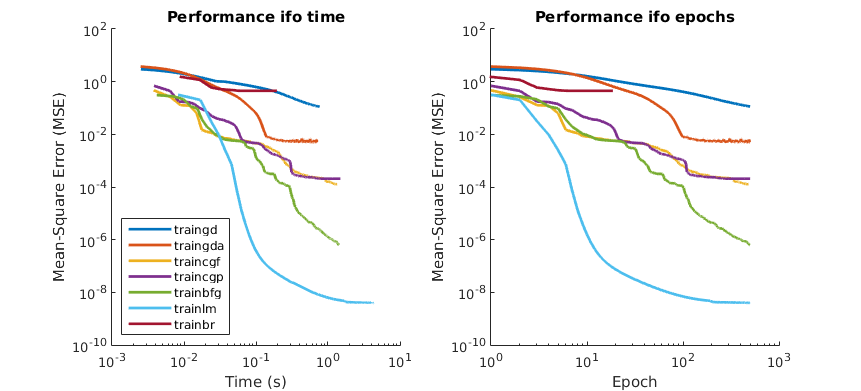
\includegraphics[width=0.9\textwidth]{figs/performance_plot.png}
\caption{Performance (MSE) of the tested training rules as a function of (left) time and (right) epochs where the maximum epochs is limited to $1000$. The log-log scale is opted to vizualize the initial drop in MSE. \label{fig:performace_plot}}
\end{figure}

Below I compare the speed of various learning schemes, compared to the most basic gradient descent algorithm. I use the abbreviations of the algorithms, as used in the assignment.

\textbf{[traingd]} The gradient descent algorithm does not perform too well for most of the tested functions. The speed of each iteration evaluation is fast, but convergence is slow, and mostly never reached within $1000$ epochs. It is clear from the broad shoulder in the performance graph in Fig.~\ref{fig:performace_plot}, that an adaptive learning rate could significantly reduce the required time for convergence.

\textbf{[traingda]} For fixed step-size gradient descent, we made the following observation: if the learning rate  is set too high, the algorithm can oscillate and become unstable. If the learning rate is too small, the algorithm takes too long to converge. An adaptive algorithm can is an attempt to provide the best of both worlds by keeping the step size as large as possible, while allowing for smaller step sizes for locally complex error surfaces. This change is based on the performance of the network in the preceding epoch. 
In the first few ($\sim 10$) epochs, the performance is very similar, yet, due to the adaptive learning rate, the MSE is reduced significantly after $100$ epochs, compared to traingd. This is reflected in an improved function approximation. Hence, approximate convergence is reached after fewer epochs. The speed of an iteration is approximately the same as for the non-adaptive gradient descent. 

\textbf{[traingdm]} Momentum softens the learning algorithms' dependence on the small local variations of the error surface. It allows to jump out of a local minimum, while other methods get stuck.

\textbf{[trainbfg]} This quasi-Newton method beats traingda by orders of magnitude (even after $10$ epochs, a clear difference is observed). Quasi-Newton methods builds up second-order derivative information, based upon gradient information during the iteration process, allowing for faster convergence, while limiting the computational overhead.

\textbf{[traincgf]} and \textbf{[traincgp]} The conjugate gradient algorithms are usually much faster than variable learning rate backpropagation. The considered conjugate-gradient methods perform very similar on the considered example. They only differ in the factor that determines the amount of influence of the momentum term in determining the next search direction. Then the next search direction is determined so that it is conjugate to previous search directions. These methods converge after just a few epochs, and combine this with a fast iteration step.

\textbf{[trainlm]} The Levenberg - Marquardt algorithm can be viewed as an adaptive mixture of a Newton-like and steepest-descent algorithm. By varying the $\lambda$ parameter in the step size $\Delta x = - (H + \lambda I)^-1 g$, one can change which algorithm is dominant. The $\lambda$ is decreased after each successful step, converging towards Newton's method which allows for fast and accurate convergence close to an error minimum. This is clearly visible in the the performance plot in Fig.~\ref{fig:performace_plot}. When for a given $\lambda$ a the step would increase the error value, the $\lambda$ is increased such that the error is always reduced. For the MSE function that is used in the network discussed here, an efficient approximation for the Hessian $H$ can be computed from the Jacobian matrix, which can be calculated much more efficiently. Altogether, the algorithms design leads to a significant overhead in the speed of each epoch (factor of $\sim 10$ compared to traingd). However, the computational cost is fully justified, since for a minimum number of epochs, function \eqref{eq:myfunction} is properly approximated.
From the above analysis, the Levenberg - Marquardt algorithm shows to be the most suitable training rule to approximate function \eqref{eq:myfunction}, given the neural network architecture and the MSE error function. It is also the default algorithm of the \texttt{feedforwardnet} object.

\section{Generalization: noisy data and overfitting}
To simulate noisy data, I add a normally distributed noise to the original dataset, with standard deviation $\sigma = 0.1$. I map the bias and variance of the various methods considered in the previous section. This is done by generating $100$ data sets, and training the considered version of the network with a given learning rule. 
\begin{figure}[hbt]
\centering
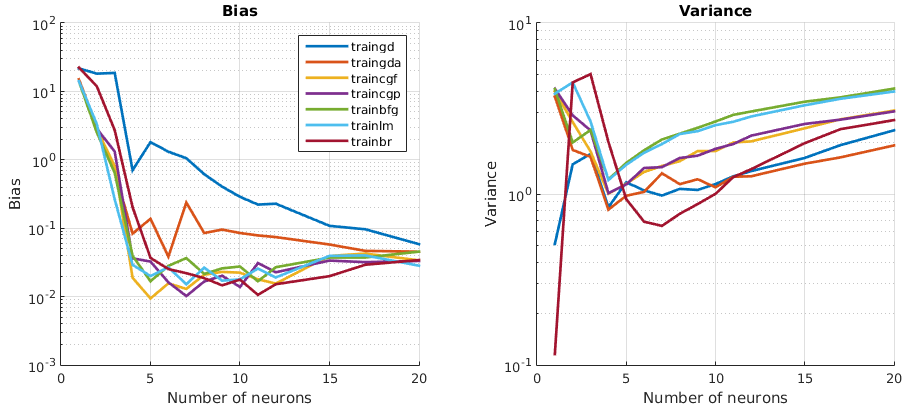
\includegraphics[width=0.9\textwidth]{figs/bias_and_variance.png}
\caption{Bias and variance as a function of the complexity of the neural network. In this exercise, \texttt{trainbr} can be ignored, since it is discussed in the next report.\label{fig:bias_and_variance}}
\end{figure}

Due to the fast learning property of the Levenberg - Marquardt algorithm, it now also requires more care to avoid overfitting. This is indicated by the large variance in Fig.~\ref{fig:bias_and_variance}. The more the network overfits the data, the larger the variation within the ensemble of networks, and the less generalizable it is. This can be avoid by e.g.\ early stopping, regularization or cross validation. More general, it appears that for different learning rules, with the same architecture and cost-function, the chance of overfitting is possitively correlated with the speed of convergence (which was the topic of the previous section). Since `a strategy to avoid overfitting' is the topic of the next report, I refer the reader to that report for more details.
\end{document}